\documentclass[tikz,border=10pt]{standalone}
\usepackage{amsmath}
\usepackage[utf8]{inputenc}
\usetikzlibrary{arrows.meta, calc, angles, quotes, decorations.pathreplacing}

\begin{document}
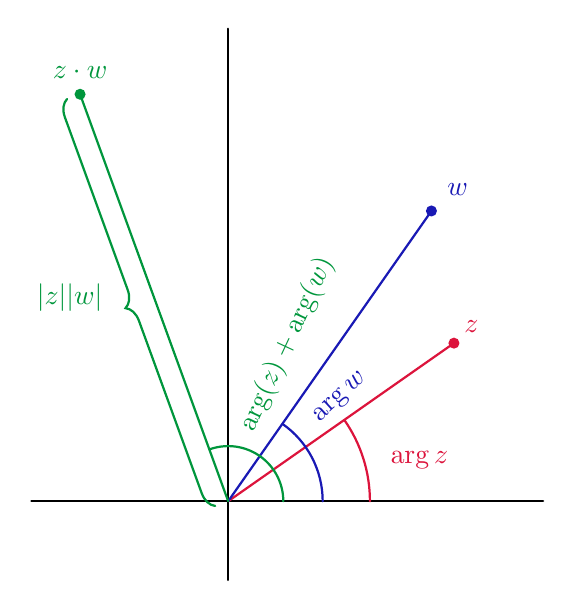
\begin{tikzpicture}[>=Stealth, thick, line cap=round]

    % --- Definitions ---
    % Colors to match the image
    \definecolor{myred}{RGB}{220, 20, 60}
    \definecolor{myblue}{RGB}{25, 25, 180}
    \definecolor{mygreen}{RGB}{0, 150, 60}

    % Coordinates (Polar: angle:radius)
    \def\angZ{35}   % Red angle
    \def\lenZ{3.5}
    
    \def\angW{55}   % Blue angle
    \def\lenW{4.5}
    
    \def\angZW{110} % Green angle = sum
    \def\lenZW{5.5} % Schematic length for z*w

    \coordinate (O) at (0,0);
    \coordinate (X) at (4,0); % Reference for angles
    
    \coordinate (Z) at (\angZ:\lenZ);
    \coordinate (W) at (\angW:\lenW);
    \coordinate (ZW) at (\angZW:\lenZW);

    % --- Axes ---
    \draw[black] (-2.5,0) -- (4.0,0); % x-axis
    \draw[black] (0,-1.0) -- (0,6); % y-axis

    % --- Vectors and Points ---
    
    % Red Vector (z)
    \draw[, myred] (O) -- (Z);
    \fill[myred] (Z) circle (2pt);
    \node[myred, anchor=south west] at (Z) {$z$};

    % Blue Vector (w)
    \draw[, myblue] (O) -- (W);
    \fill[myblue] (W) circle (2pt);
    \node[myblue, anchor=south west, xshift=2pt, yshift=2pt] at (W) {$w$};

    % Green Vector (z.w)
    \draw[, mygreen] (O) -- (ZW);
    \fill[mygreen] (ZW) circle (2pt);
    \node[mygreen, anchor=south, yshift=2pt] at (ZW) {$z \cdot w$};
    
    % --- Green Bracket and Label ---
    % Label is now horizontal (no 'sloped') and positioned to the left
    \draw[decorate, decoration={brace, amplitude=6pt, raise=5pt}, mygreen] 
        (O) -- (ZW) 
        node[midway, left=15pt, mygreen] {$|z||w|$};

    % --- Angles and Labels ---

    % 1. Red Angle (arg z)
    \draw[myred] (1.8,0) arc (0:\angZ:1.8);
    \node[myred, anchor=west] at (15:2.0) {$\arg z$};

    % 2. Blue Angle (arg w)
    \draw[myblue] (1.2,0) arc (0:\angW:1.2);
    \node[myblue, rotate=\angW/2+15, anchor=west] at (\angW/2+15:1.4) {$\arg w$};

    % 3. Green Angle (arg(z) + arg(w))
    \draw[mygreen] (0.7,0) arc (0:\angZW:0.7);
    \node[mygreen, rotate=\angZW/2+10, anchor=south west] at (\angZW/2:0.8) {$\arg(z)+\arg(w)$};

\end{tikzpicture}
\end{document}
